\documentclass[border=10pt]{standalone}

\usepackage[utf8]{inputenc}                                 % Codificação do documento
\usepackage[T1]{fontenc}                                    % Seleção de código de fonte
\usepackage{microtype}                                      % Melhora a justificação do documento
\usepackage{lmodern}                                        % Usa a fonte Latin Modern
\usepackage{ae, aecompl}                                    % Fontes de alta qualidade

\usepackage{amsmath}
\usepackage{verbatim}
\usepackage{tikz}
\usetikzlibrary{arrows,calc,positioning,shadows.blur,decorations.pathreplacing}
\usepackage{etoolbox}

\usepackage{fontawesome}

\begin{document}
\begin{tikzpicture}
[
	              y = -1cm,
	           ->, >= stealth',
	  node distance = 2cm,
	  vertex/.style = { draw=black, circle, inner sep=2.5pt },
         dot/.style = { draw=black, fill=black, circle, inner sep=0.75pt },
	   label/.style = { draw=none, fill=none, anchor=west },
	toplabel/.style = { draw=none, fill=none, anchor=south }
]
	\node (AppFolder)       at (  0,  0)    [label]     {\faFolderOpen};
	\node (AppLabel)        at (0.5,  0)    [label]     {\texttt{App}};
    \node[white] (AppEdge)  at (  0,5.9)    [label]     {\faFolderOpen};
	\draw[-] (AppFolder) edge[opacity=0.4] (AppEdge);

        \node (StoreFolder)         at (0.5,0.5)    [label]     {\faFolderOpen};
        \node (StoreLabel)          at (  1,0.5)    [label]     {\texttt{Store}};
        \node[white] (StoreEdge)    at (0.5,3.4)    [label]     {\faFolderOpen};
	    \draw[-] (StoreFolder) edge[opacity=0.4] (StoreEdge);

            \node (CartFile)                    at (  1,  1)    [label]     {\faFileText};
            \node (CartLabel)                   at (1.5,  1)    [label]     {\texttt{Cart}};
            \node[white] (CartEdge)             at (  1,2.4)    [label]     {\faFileText};
	        \draw[-] (CartFile) edge[opacity=0.4] (CartEdge);

                \node (GetCartFunction)             at (1.5,1.5)    [label]     {\textit{fn}};
                \node (GetCartLabel)                at (  2,1.5)    [label]     {\texttt{GetCart}};
                \node (ShowCartFunction)            at (1.5,  2)    [label]     {\textit{fn}};
                \node (ShowCartLabel)               at (  2,  2)    [label]     {\texttt{ShowCart}};

                \draw (6,1.95) -- (7,1.95) -- (7,1.5) -> (6,1.5);

            \node (FeaturedItemsFile)           at (  1,2.5)    [label]     {\faFileText};
            \node (FeaturedItemsLabel)          at (1.5,2.5)    [label]     {\texttt{FeaturedItems}};
            \node[white] (FeaturedItemsEdge)    at (  1,3.4)    [label]     {\faFileText};
	        \draw[-] (FeaturedItemsFile) edge[opacity=0.4] (FeaturedItemsEdge);

                \node (ShowFeaturedItemsFunction)   at (1.5,  3)    [label]     {\textit{fn}};
                \node (ShowFeaturedItemsLabel)      at (  2,  3)    [label]     {\texttt{ShowFeaturedItems}};

        \node (UsersFolder)         at (0.5,3.5)    [label]     {\faFolderOpen};
        \node (UsersLabel)          at (  1,3.5)    [label]     {\texttt{Users}};
        \node[white] (UsersEdge)    at (0.5,4.9)    [label]     {\faFolderOpen};
	    \draw[-] (UsersFolder) edge[opacity=0.4] (UsersEdge);

            \node (SessionFile)             at (  1,  4)    [label]     {\faFileText};
            \node (SessionLabel)            at (1.5,  4)    [label]     {\texttt{Session}};
            \node[white] (SessionEdge)      at (  1,4.9)    [label]     {\faFileText};
	        \draw[-] (SessionFile) edge[opacity=0.4] (SessionEdge);

                \node (GetSessionFunction)          at (1.5,4.5)    [label]     {\textit{fn}};
                \node (GetSessionLabel)             at (  2,4.5)    [label]     {\texttt{GetSession}};

        \node (MainFile)        at (0.5,  5)    [label]     {\faFileText};
        \node (MainLabel)       at (  1,  5)    [label]     {\texttt{Main}};
        \node[white] (MainEdge) at (0.5,5.9)    [label]     {\faFileText};
	    \draw[-] (MainFile) edge[opacity=0.4] (MainEdge);

            \node (MainFunction)      at (  1,5.5)    [label]     {\textit{fn}};
            \node (MainLabel)         at (1.5,5.5)    [label]     {\texttt{Main}};

            \draw (6,5.5)   -- (7,5.5) -- (7,4.5) -> (6,4.5);
            \draw (7,4.5) -- (7,3)   -> (6,3);
            \draw (7,3)   -- (7,2.05)   -> (6,2.05);
            \node at (7,3) [dot] {};

\end{tikzpicture}
\end{document}